\documentclass[12pt,a4paper]{article}

\usepackage[utf8]{inputenc}
\usepackage[brazilian]{babel}
\usepackage{amsmath}
\usepackage{graphicx}
\usepackage{siunitx}
\usepackage{booktabs}
\usepackage{geometry}
\usepackage{float}
\usepackage{indentfirst}

\usepackage[authoryear]{natbib}

\geometry{margin=2.5cm}

\title{Determinação de constantes elásticas de molas por meio de associação em série e paralelo}
\author{Enzo Rocha Leite Diniz Ribas \\ Centro Federal de Educação Tecnológica de Minas Gerais}
\date{\today}

\begin{document}
\begin{titlepage}

\begin{center}


\includegraphics[width=4cm]{media/Logo_CEFET-MG.png}

\Large
Centro Federal de Educação Tecnológica de Minas Gerais

\vspace{1cm}

\Large
Curso de Engenharia Mecânica

\vspace{2cm}

\Huge
Determinação de constantes elásticas de molas por meio de associação em série e paralelo

\vspace{3cm}

\begin{flushright}
\Large
Mecânica, Oscilações, Fluidos e Termodinâmica, Turma T03 \\
Prof. Dr. Mauro Lucio Lobão Iannini
\end{flushright}

\vspace{3cm}

\large
Enzo Rocha Leite Diniz Ribas (Eng. Mecânica - 20253002819)\\
Gabriel Resende Amorim Oliveira (Eng. Elétrica - 20233014438)\\
Leandro Césari e Silva Barros (Eng. Mecânica - 20253005104)\\

\vfill

\Large
Belo Horizonte

\Large
\the\year/{1}

\end{center}

\end{titlepage}

\section{Introdução}

O roteiro do experimento \citep{Roteiro_Experimento_02} propõe a determinação de constantes elásticas de molas por meio de associações em série e paralelo.

\section{Fundamentação Teórica}


Uma mola em equilíbrio, ao sofrer uma força externa que a desloca por $x$ metros da posição de equilíbrio, exerce uma força que sempre tende a fazer a mola retornar a posição de equilíbrio. Para valores de $x$ suficientemente pequenos, a Lei de Hooke,
\begin{equation}
    F = k x,
    \label{eq:hooke}
\end{equation}
pode ser verificada experimentalmente, ou seja, \textit{a força restauradora é proporcional ao deslocamento da posição de equilíbro (linear);} \citep{moyses2013}

\section{Metodologia}

Os sistemas massa-mola, usados de forma clássica para exemplificar a Lei de Hooke \eqref{eq:hooke}, são apresentados nas figuras \ref{fig:setup1} e \ref{fig:setup2}, em situações de equilíbrio estático. \citep{Roteiro_Experimento_02}

\begin{figure}[H]
\centering
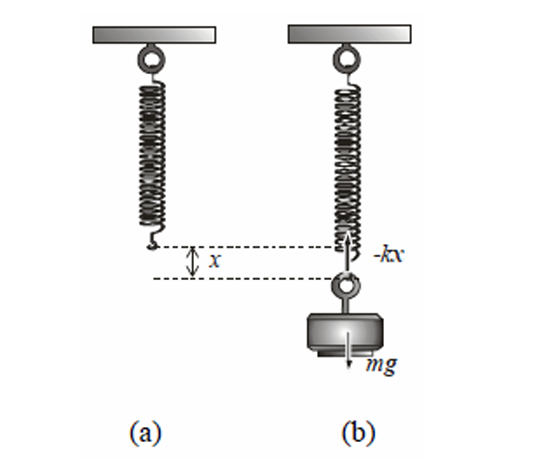
\includegraphics[width=0.7\textwidth]{media/photos/spring_diagram1.png}
\caption{Uma mola helicoidal de massa desprezível é pendurada por uma extremidade (a). Ao se 
colocar um objeto de massa  na outra extremidade, ocorre um alongamento (b).  Fonte: \citep{Roteiro_Experimento_02}.}
\label{fig:setup1}
\end{figure}


\begin{figure}[H]
\centering
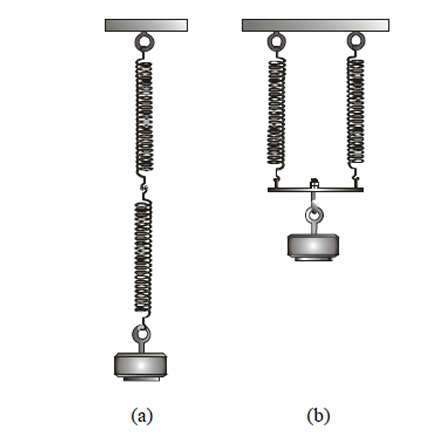
\includegraphics[width=0.7\textwidth]{media/photos/spring_diagram2.png}
\caption{Ilustração da associação de duas molas (a) em série, com uma posicionada na 
extremidade da outra, e (b) em paralelo, com uma posicionada ao lado da outra. Fonte: \citep{Roteiro_Experimento_02}.}
\label{fig:setup2}
\end{figure}

A partir da variação da massa presa à mola e do deslocamento da distenção, os sistemas descritos foram realizados experimentos para determinar as constantes elásticas de duas molas como exemplificado na Figura \ref{fig:setup3}. 

\begin{figure}[H]
\centering
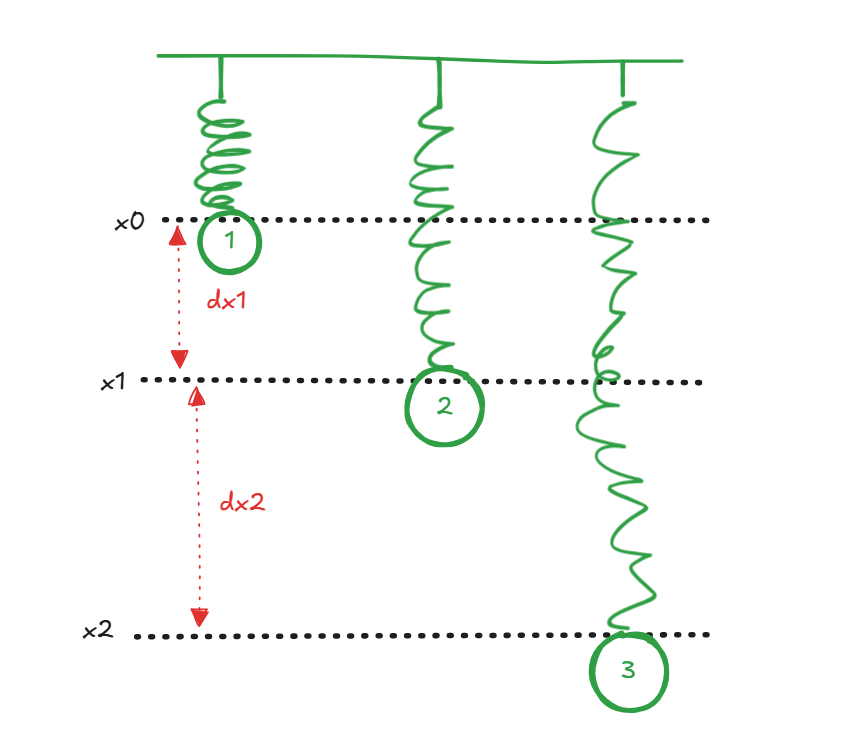
\includegraphics[width=0.7\textwidth]{media/photos/spring_diagram3.png}
\caption{Exemplificação da variação da massa presa à mola e do deslocamento da distenção. Fonte: Autor.}
\label{fig:setup3}
\end{figure}

O sistema da figura \ref{fig:setup1} é usado para determinar a constante elástica $k_1$ de uma mola. Enquanto o sistema da figura \ref{fig:setup2} é usado para determinar a constante elástica $k_{s}$ da associação em série e $k_{p}$ da associação em paralelo. As massas utilizadas para variar o peso do sistema não foram devidamente calibradas, o que pode levar a leves desvios nos resultados, mas não significativos para a finalidade do experimento. 

Com o sistema montado, foram selecionadas duas molas, \textit{mola 1} e \textit{mola 2}, com constantes elásticas $k_1$ e $k_2$, respectivamente. Com o setup da figura \ref{fig:setup1} foi observado o deslocamento da mola com a variação do peso, e registrado. Em seguida, com o setup da figura \ref{fig:setup2} foram observados os deslocamentos para as associações em série e paralelo de $k_1$ e $k_2$, e registrados.

A partir da análise dos dados obtidos, as constantes elásticas da \textit{mola 1}, $k_1$; do sistema em série, $k_s$ e do sistema em paralelo, $k_p$ foram determinadas, e a constante elástica $k_2$ da segunda mola foi calculada a partir das relações de associação em série e paralelo. Ademais a constante elástica $k_2$ da segunda mola também foi determinada a partir do setup da figura \ref{fig:setup1} para comparação com o valor calculado a partir das associações em série e paralelo.

\section{Procedimentos}

O procedimento experimental seguiu as seguintes etapas:

\subsubsection{Ajuste de posições do sistema}
As molas foram fixadas em um suporte vertical, garantindo que estivessem alinhadas e livres para se estenderem sem obstruções. Suas posições iniciais foram marcadas para referência.

\subsubsection{Variação da massa e registro do deslocamento}
Foram utilizadas massas diferentes para variar o peso do sistema, e os deslocamentos das molas foram registrados.

\subsubsection{Repetição das medições para diferentes massas e associações}
Foram feitas medições para diferentes massas e para as associações em série e paralelo, garantindo a obtenção de um conjunto de dados robusto para análise.

\subsubsection{Organização dos dados em tabela}
Os dados coletados foram organizados em tabelas para facilitar a análise. Cada tabela continha as massas utilizadas, os deslocamentos correspondentes e a força peso associada a cada massa, calculada como $F = mg$, em que $g$ é a aceleração da gravidade local ($g_{bh} = 9.78 \, \text{m/s}^2$).

\subsubsection{Construção de gráficos e realização de ajustes no SciDAVis}
Os dados organizados em tabela foram importados para o software SciDAVis para análise de dados. Gráficos de força peso $F$ versus deslocamento $x$ foram construídos para cada configuração (mola 1, mola 2, série e paralelo). Ajustes lineares foram realizados para determinar as constantes elásticas a partir do coeficiente angular dos gráficos, utilizando a relação 

\begin{equation}
    k = \frac{F}{x}.
\end{equation}

\subsubsection{Cálculo das constantes elásticas}
A partir dos coeficientes dos ajustes lineares calculados experimentalmente, as constantes elásticas $k_1$, $k_2$, $k_s$ e $k_p$ foram determinadas.

A partir da análise do diagrama de corpo livre, as relações de associação em série e paralelo foram utilizadas para calcular a constante elástica $k_2$ da segunda mola, e os resultados foram comparados com o valor obtido diretamente do ajuste linear do setup da figura \ref{fig:setup1}.

No sistema em paralelo as molas estão sujeitas à mesma força peso, o que causa o mesmo deslocamento nas duas. Pela lei de Hooke, a força em cada mola é dada por $F_1 = k_1 x$ e $F_2 = k_2 x$. A força total é a soma das forças individuais, ou seja, $F = F_1 + F_2 = (k_1 + k_2)x$. Assim, a constante elástica equivalente para o sistema em paralelo é dada por
\begin{equation}
    k_p = k_1 + k_2.
    \label{eq:parallel}
\end{equation}
Já no sistema em série, a força é a mesma em ambas as molas, ou seja, $F_T = F_1 = F_2$. O deslocamento total é a soma dos deslocamentos individuais, ou seja, $x_T = x_1 + x_2$. Pela lei de Hooke, temos $x_1 = \frac{F_T}{k_1}$ e $x_2 = \frac{F_T}{k_2}$. Assim, o deslocamento total é dado por

\begin{equation*}
    x_T = \frac{F_T}{k_1} + \frac{F_T}{k_2} = F_T\left(\frac{1}{k_1} + \frac{1}{k_2}\right).
\end{equation*}
A constante elástica equivalente para o sistema em série é dada por
\begin{equation}
    k_s = \frac{F_T}{x_T} = \frac{F_T}{F_T\left(\frac{1}{k_1} + \frac{1}{k_2}\right)} = \frac{1}{\frac{1}{k_1} + \frac{1}{k_2}} = \frac{k_1 k_2}{k_1 + k_2}.
    \label{eq:series}
\end{equation}

Com esses resultados, é possível perceber que a constante elástica em paralelo é sempre maior do que a constante elástica de cada mola individualmente, enquanto a constante elástica em série é sempre menor do que a constante elástica de cada mola individualmente.

\section{Discussão e Análise dos Resultados}

\subsection{Constante da Mola 1}

A Tabela ~\ref{tab:table_spring1} apresenta os valores experimentais obtidos para a \textit{mola 1} com o sistema \ref{fig:setup1}.

\begin{table}[H]
\centering
\begin{tabular}{S[table-format=0.3] S[table-format=1.3] S[table-format=1.3]}
\toprule
\multicolumn{1}{c}{\shortstack{\textbf{Deslocamento da mola} \\ \textbf{$x \pm 0,005$ (m)}}} & \multicolumn{1}{c}{\shortstack{\textbf{Variação da massa} \\ \textbf{$\Delta m$ (kg)}}} & \multicolumn{1}{c}{\shortstack{\textbf{Variação da força peso} \\ \textbf{$F \pm 0,005$ (N)}}} \\
\midrule
0     & 0     & 0,0 \\
0,025 & 0,05 & 0,489 \\
0,05  & 0,10 & 0,978 \\
0,075 & 0,15 & 1,467 \\
0,1   & 0,20 & 1,956 \\
0,125 & 0,25 & 2,445 \\
0,15  & 0,30 & 2,934 \\
\bottomrule
\end{tabular}
\caption{Dados experimentais de deslocamento da \textit{mola 1}, variação da massa e força peso.}
\label{tab:table_spring1}
\end{table}

O gráfico da força peso em função do deslocamento da mola, ilustrado na Figura ~\ref{graph1_spring1}, apresenta um comportamento linear, conforme esperado teoricamente.

\begin{figure}[H]
\centering
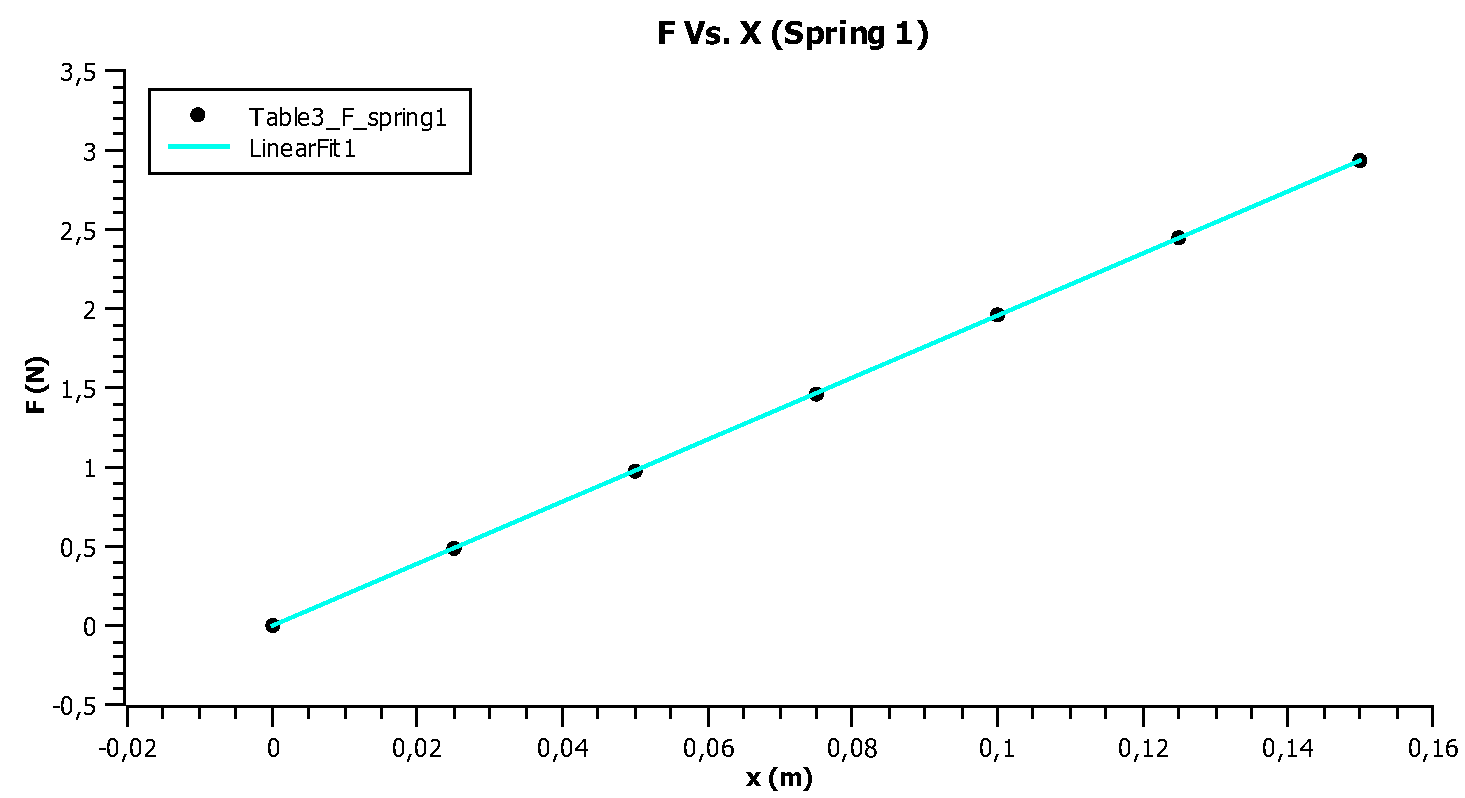
\includegraphics[width=0.7\textwidth]{media/graph_spring1}
\caption{Gráfico da força peso em função do deslocamento da mola 1.}
\label{graph1_spring1}
\end{figure}

\subsubsection{Log do SciDAVis}
\begin{verbatim}
[domingo, 5 de abril de 2026 20:46:14 Hora oficial do Brasil	Plot: ''Graph1'']
Linear Regression fit of dataset: Table3_F_spring1, using function: A*x+B
Y standard errors: Unknown
From x = 0 to x = 0,15
B (y-intercept) = -5,55111512312578e-17 +/- 5,0037075531084e-17
A (slope) = 19,56 +/- 1,14919000872408e-15
--------------------------------------------------------------------------------------
Chi^2 = 1,76338145708095e-30
R^2 = 1
---------------------------------------------------------------------------------------
\end{verbatim}

O coeficiente angular do ajuste linear, $A$, representa a constante elástica $k_1$ da \textit{mola 1}, resultando em
\begin{equation}
    k_1 = 19,56 \pm 1,15 \times 10^{-15}  \text{ N/m}
    \label{k1_linearfit}
\end{equation}

\subsection{Constante da Associação em Série}

A Tabela ~\ref{tab:table_ass_series} apresenta os valores experimentais obtidos para a associação em série das molas.

\begin{table}[H]
\centering
\begin{tabular}{S[table-format=0.3] S[table-format=1.3] S[table-format=1.3]}
\toprule
\multicolumn{1}{c}{\shortstack{\textbf{Deslocamento da mola} \\ \textbf{$x \pm 0,005$ (m)}}} & \multicolumn{1}{c}{\shortstack{\textbf{Variação da massa} \\ \textbf{$\Delta m$ (kg)}}} & \multicolumn{1}{c}{\shortstack{\textbf{Variação da força peso} \\ \textbf{$F \pm 0,005$ (N)}}} \\
\midrule
0,77  & 0,0  & 0,00 \\
0,807 & 0,01 & 0,0978 \\
0,84  & 0,02 & 0,1956 \\
0,878 & 0,03 & 0,2934 \\
0,916 & 0,04 & 0,3912 \\
0,952 & 0,05 & 0,489 \\
\bottomrule
\end{tabular}
\caption{Dados experimentais da associação em série}
\label{tab:table_ass_series}
\end{table}

O gráfico da força peso em função do deslocamento da associação em série, ilustrado na Figura ~\ref{graph_series_ass}, apresenta um comportamento linear, conforme esperado teoricamente.

\begin{figure}[H]
\centering
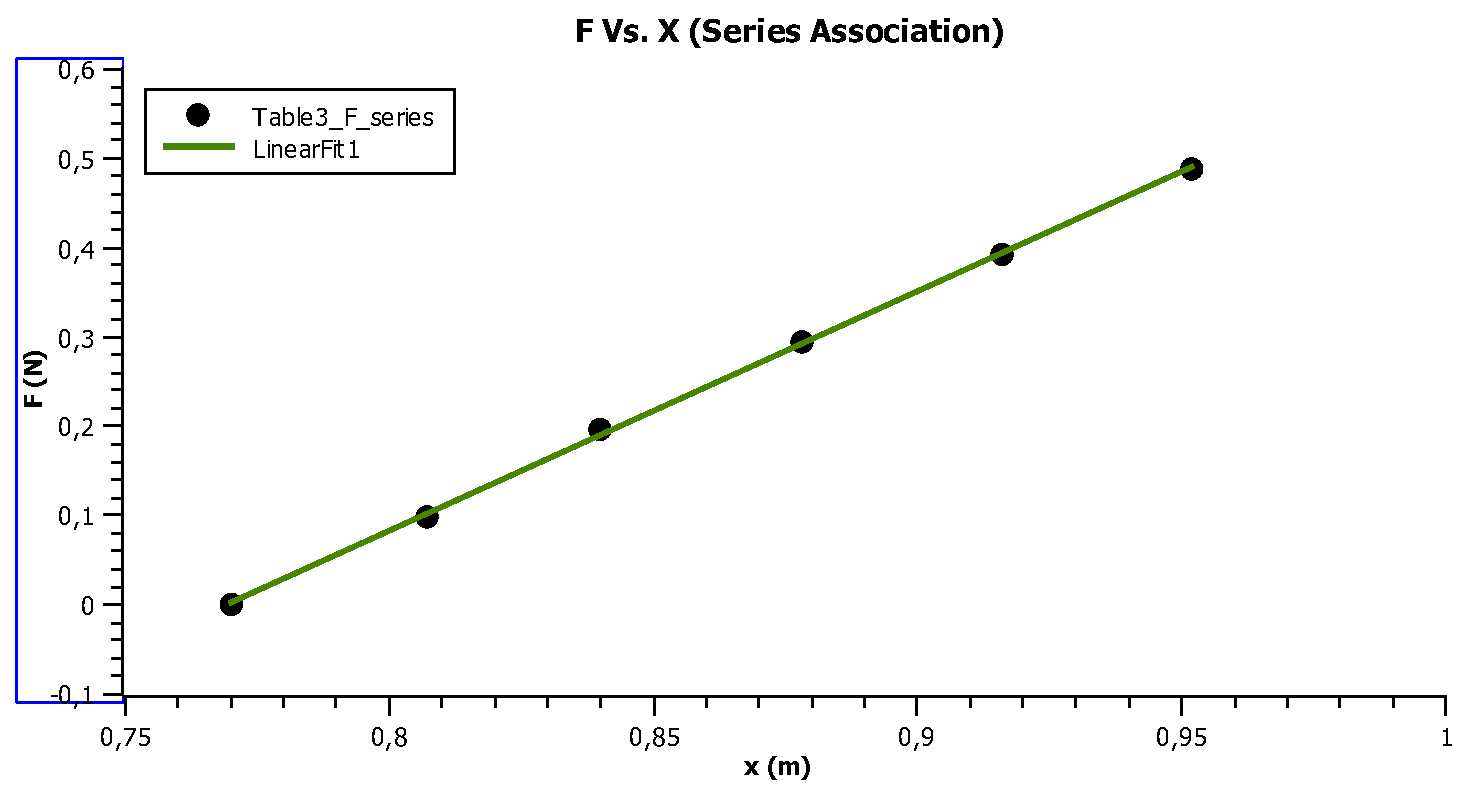
\includegraphics[width=0.7\textwidth]{media/graph_series_ass}
\caption{Gráfico da força peso em função do deslocamento da associação em série.}
\label{graph_series_ass}
\end{figure}

\subsubsection{Log do SciDAVis}
\begin{verbatim}
[domingo, 5 de abril de 2026 20:46:25 Hora oficial do Brasil	Plot: ''Graph5'']
Linear Regression fit of dataset: Table3_F_series, using function: A*x+B
Y standard errors: Unknown
From x = 0,77 to x = 0,952
B (y-intercept) = -2,0648654628414 +/- 0,0218674932954764
A (slope) = 2,68374835890924 +/- 0,0253463605407724
--------------------------------------------------------------------------------------
Chi^2 = 5,96991929061857e-05
R^2 = 0,99988651771791
---------------------------------------------------------------------------------------
\end{verbatim}

O coeficiente angular do ajuste linear, $A$, representa a constante elástica $k_s$ da associação em série, resultando em
\begin{equation}
    k_s = 2,68 \pm 0,02 \text{ N/m}
    \label{k_series_linearfit}
\end{equation}

\subsection{Constante da Associação em Paralelo}

A Tabela ~\ref{tab:table_ass_parallel} apresenta os valores experimentais obtidos para a associação em paralelo das molas.

\begin{table}[H]
\centering
\begin{tabular}{S[table-format=0.3] S[table-format=1.3] S[table-format=1.3]}
\toprule
\multicolumn{1}{c}{\shortstack{\textbf{Deslocamento da mola} \\ \textbf{$x \pm 0,005$ (m)}}} & \multicolumn{1}{c}{\shortstack{\textbf{Variação da massa} \\ \textbf{$\Delta m$ (kg)}}} & \multicolumn{1}{c}{\shortstack{\textbf{Variação da força peso} \\ \textbf{$F \pm 0,005$ (N)}}} \\
\midrule
0	 & 0	 & 0,0 \\
0,019 & 0,05 & 0,489 \\
0,040 & 0,10 & 0,978 \\
0,063 & 0,15 & 1,467 \\
0,084 & 0,20 & 1,956 \\
0,105 & 0,25 & 2,445 \\
0,120 & 0,30 & 2,934 \\
\bottomrule
\end{tabular}
\caption{Dados experimentais da associação em paralelo}
\label{tab:table_ass_parallel}
\end{table}

O gráfico da força peso em função do deslocamento da associação em paralelo, ilustrado na Figura ~\ref{graph_parallel_ass}, apresenta um comportamento linear, conforme esperado teoricamente.

\begin{figure}[H]
\centering
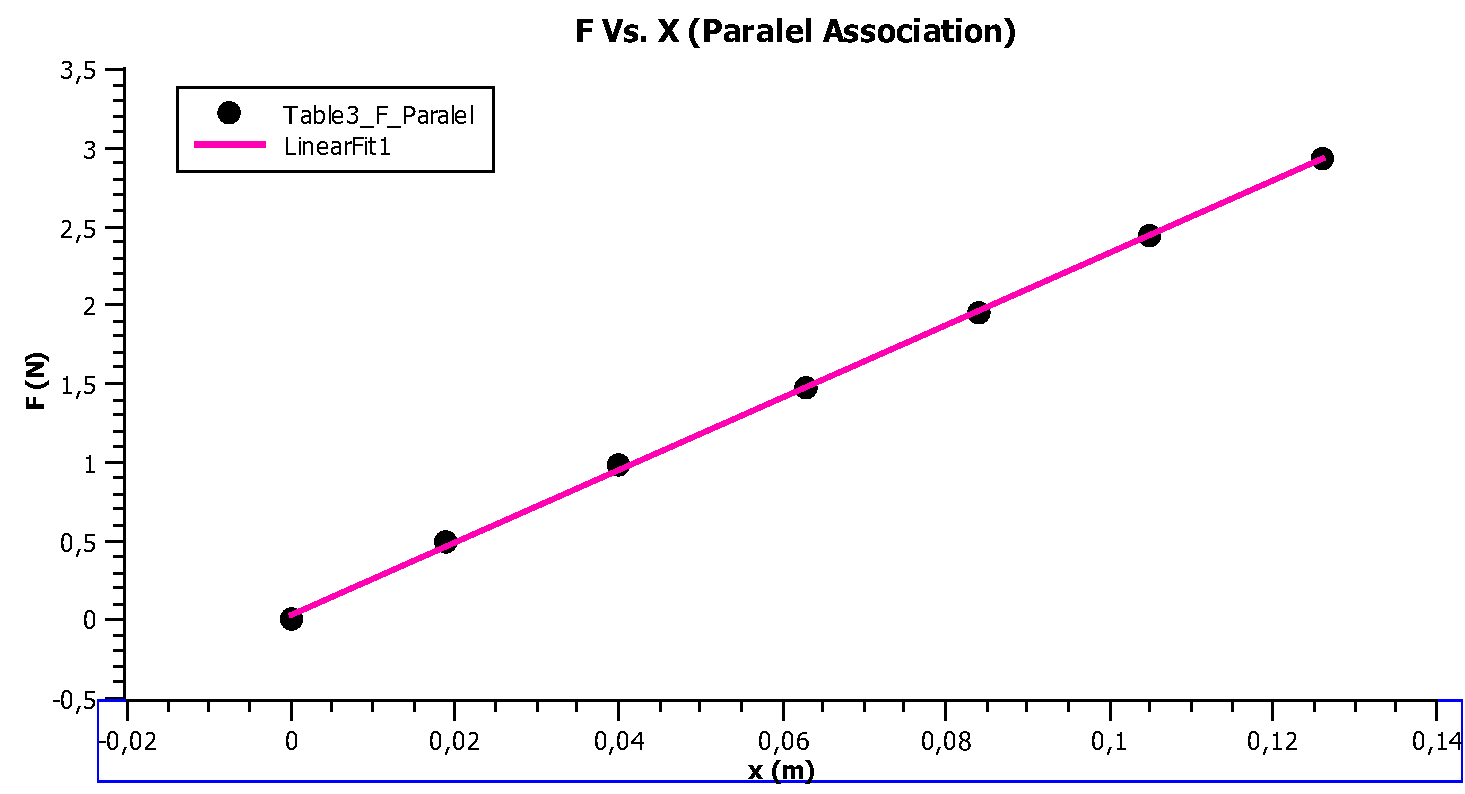
\includegraphics[width=0.7\textwidth]{media/graph_paralel_ass}
\caption{Gráfico da força peso em função do deslocamento da associação em paralelo.}
\label{graph_parallel_ass}
\end{figure}

\subsubsection{Log do SciDAVis}
\begin{verbatim}
[domingo, 5 de abril de 2026 20:46:29 Hora oficial do Brasil	Plot: ''Graph2'']
Linear Regression fit of dataset: Table3_F_Paralel, using function: A*x+B
Y standard errors: Unknown
From x = 0 to x = 0,126
B (y-intercept) = 0,0284954442429732 +/- 0,014582564522473
A (slope) = 23,0424070716229 +/- 0,193182258947935
--------------------------------------------------------------------------------------
Chi^2 = 0,00235218753399807
R^2 = 0,99989190320106
---------------------------------------------------------------------------------------
\end{verbatim}

O coeficiente angular do ajuste linear, $A$, representa a constante elástica $k_p$ da associação em paralelo, resultando em
\begin{equation}
    k_p = 23,04 \pm 0,19 \text{ N/m}
    \label{k_parallel_linearfit}
\end{equation}

\subsection{Constante da Mola 2}

A Tabela ~\ref{tab:table_spring2} apresenta os valores experimentais obtidos para a \textit{mola 2} com o sistema \ref{fig:setup1}.

\begin{table}[H]
\centering
\begin{tabular}{S[table-format=0.3] S[table-format=1.3] S[table-format=1.3]}
\toprule
\multicolumn{1}{c}{\shortstack{\textbf{Posição da mola} \\ \textbf{$x \pm 0,005$ (m)}}} & \multicolumn{1}{c}{\shortstack{\textbf{Variação da massa} \\ \textbf{$\Delta m$ (kg)}}} & \multicolumn{1}{c}{\shortstack{\textbf{Variação da força peso} \\ \textbf{$F \pm 0,005$ (N)}}} \\
\midrule
0,544 & 0 &	0 \\
0,695 &	0,05 & 0,489 \\
0,848 &	0,10 & 0,978 \\
0,878 &	0,11 & 1,0758 \\
0,881 &	0,111 & 1,08558 \\
\bottomrule
\end{tabular}
\caption{Dados experimentais da \textit{mola 2}, variação da massa e força peso.}
\label{tab:table_spring2}
\end{table}


O gráfico da força peso em função do deslocamento da mola, ilustrado na Figura ~\ref{graph1_spring2}, apresenta um comportamento linear, conforme esperado teoricamente.

\begin{figure}[H]
\centering
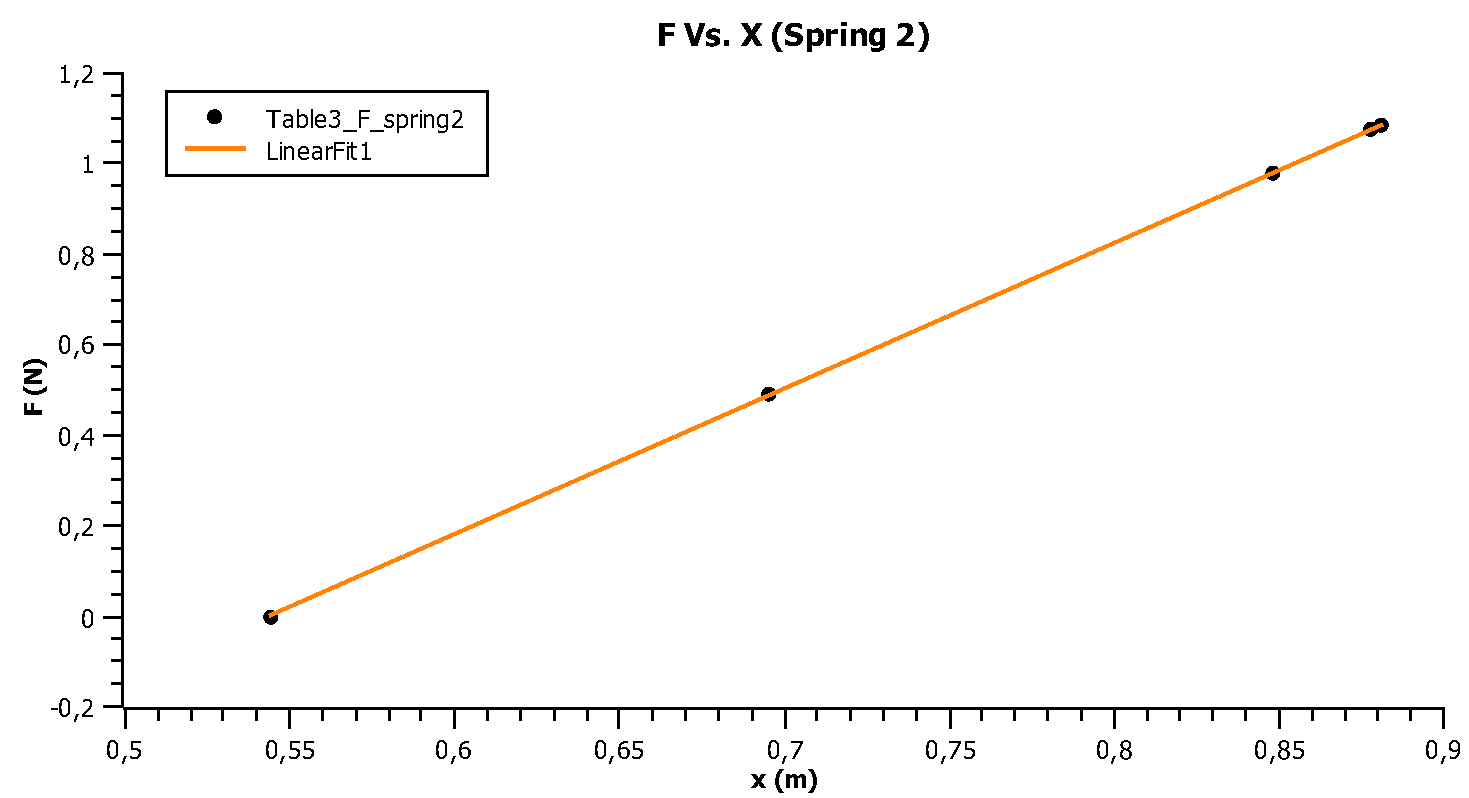
\includegraphics[width=0.7\textwidth]{media/graph_spring2}
\caption{Gráfico da força peso em função do deslocamento da mola 2.}
\label{graph1_spring2}
\end{figure}

\subsubsection{Log do SciDAVis}
\begin{verbatim}
[domingo, 5 de abril de 2026 20:46:32 Hora oficial do Brasil	Plot: ''Graph4'']
Linear Regression fit of dataset: Table3_F_spring2, using function: A*x+B
Y standard errors: Unknown
From x = 0,544 to x = 0,881
B (y-intercept) = -1,74944933241747 +/- 0,00403552743533766
A (slope) = 3,21779164380846 +/- 0,00517111044550637
--------------------------------------------------------------------------------------
Chi^2 = 6,96053245342771e-06
R^2 = 0,99999802897879
---------------------------------------------------------------------------------------
\end{verbatim}

O coeficiente angular do ajuste linear, $A$, representa a constante elástica $k_2$ da \textit{mola 2}, resultando em
\begin{equation}
    k_2 = 3,21 \pm 0,005 \text{ N/m}
    \label{eq:k2_linearfit}
\end{equation}


\subsection{Discussão dos Resultados}

Assim como esperado teoricamente, os gráficos da força peso em função do deslocamento da mola 1, da associação em série e da associação em paralelo apresentaram um comportamento linear, o que é consistente com a Lei de Hooke \eqref{eq:hooke}. Os ajustes lineares realizados para cada configuração permitiram a determinação das constantes elásticas $k_1$, $k_s$, $k_p$ e $k_2$ a partir dos coeficientes angulares dos gráficos. Confirmando a relação as relações de que a associação em paralelo resulta em uma constante elástica maior do que a constante elástica de cada mola individualmente, enquanto a associação em série resulta em uma constante elástica menor do que a constante elástica de cada mola individualmente.

\section{Análise dos Resultados}


\subsection{Concordância com o Valor de Referência}

Utilizando os modelos das equações \eqref{eq:series} e \eqref{eq:parallel}, com base nos resultados obtidos experimentalmente para as constantes elásticas $k_1$, $k_s$ e $k_p$, foi possível calcular a constante elástica $k_2$ da segunda mola, e comparar com o valor obtido diretamente do ajuste linear do setup da figura \ref{fig:setup1} para $k_2$.

Pela equação \eqref{eq:parallel}, a constante elástica $k_2$ da segunda mola pode ser calculada a partir da associação em paralelo, resultando em
\begin{equation*}
    k_p = k_1 + k_2 \implies k_2 = k_p - k_1 \implies 23,00 - 19,56 = 3,44 \text{ N/m}
\end{equation*}

e pela equação \eqref{eq:series}, a constante elástica $k_2$ da segunda mola pode ser calculada a partir da associação em série, resultando em
\begin{equation*}
    k_s = \frac{k_1 k_2}{k_1 + k_2} \implies k_2 = \frac{k_s k_1}{k_1 - k_s} \implies \frac{2,68 \times 19,56}{19,56 - 2,68} = 3,105 \text{ N/m}
\end{equation*}
Em comparação com o valor obtido diretamente do ajuste linear do setup da figura \ref{fig:setup1} para $k_2$ \eqref{eq:k2_linearfit}, que resultou em $3,21 \pm 0,005$ N/m, é possível perceber que os valores calculados a partir das associações em série e paralelo apresentam uma boa concordância, com um desvio de aproximado de $7\%$ para o valor calculado a partir da associação em paralelo e um desvio aproximado de $3\%$ para o valor calculado a partir da associação em série.

\section{Conclusão}

O experimento permitiu a determinação das constantes elásticas de duas molas, bem como a análise das associações em série e paralelo. Os resultados obtidos para as constantes elásticas $k_1$, $k_s$, $k_p$ e $k_2$ apresentaram uma boa concordância com os valores esperados teoricamente, e os cálculos realizados a partir das associações em série e paralelo para determinar $k_2$ também apresentaram uma boa concordância com o valor obtido diretamente do ajuste linear do setup da figura \ref{fig:setup1} para $k_2$.

\bibliographystyle{plainnat}
\bibliography{refs}

\end{document}